\documentclass[a4paper,12pt,titlepage]{article} % [papersize,fontsize,add title page]{document type}

% This LaTeX file can be turned straight into a pdf by "PDFTeXify" in WinEdit, or
% by any LaTeX --> PDF command in another LaTeX editor
%
% Because figure files are PDF, LaTeX --> DVI does not work

% usepackage{.} reads in additional LaTeX packages
\usepackage[pdftex]{graphicx}       % to include graphs
\usepackage{natbib}                 % A BibTeX style file for references.
\usepackage{amssymb,amsmath}        % for maths symbols and equation numbering

% set up title page
\title{Title}
\author{Name \vspace{2cm} \\
Supervisor : Dr/Prof A. N. Other \vspace{2cm} \\
Department of Statistical Science \\
University College London}
\date{\today} % \today gives today's date. ... or put in the date you want

% set page size and margins
\setlength{\textwidth}{17cm}
\setlength{\textheight}{26cm}
\setlength{\oddsidemargin}{-0.5cm}
\setlength{\evensidemargin}{-0.5cm}
\setlength{\topmargin}{-25mm}
\setlength{\parindent}{0cm}
\setlength{\parskip}{0.3cm}

\let\leq=\leqslant   % for nice-looking inequality signs
\let\geq=\geqslant

\numberwithin{equation}{section}  % equation numbers like (section#.equation#)

\linespread{1}     % 1: single-spacing, 2: double-spacing, 1.5: 1.5-spacing etc

\begin{document}   % start of document
\maketitle         % create title etc
\tableofcontents   % create table of contents
\newpage           % start a new page

\section{Introduction}             % start a new section called `Introduction'
\label{sec:intro}                  % create label for this section
Write the introduction in here.    % content of the introduction

Second paragraph of the introduction \ldots  % New paragraph by leaving a blank line

\subsection{Structure of the report}         % start a new subsection
\label{sec:structure}                        % section label
In Section \ref{sec:section2} we see how to do various useful things.
In Section \ref{sec:graphs} we import pdf files.
In Section \ref{sec:tables} we create a table. %\ref{label} gives number of section called label.
In Section \ref{sec:maths} we produce some mathematics.
In Section \ref{sec:lists} we produce lists.
In Section \ref{sec:refs} we consider citing books, papers etc..

\section{Name of section 2}                      % start another new section
How to do important things like importing graphs, create tables and produce beautiful mathematics.
\label{sec:section2}                             % label for this section
\subsection{Including a pdf file as a figure}    % create a subsection
\label{sec:graphs}
Figure \ref{fig:space_dep} shows that, even for pairs of sites situated at opposite points of the network, there is strong spatial association in the storm peak values.

\begin{figure}[h]    % start of figure environment
\centering           % put the graph(s) in the centre of the page (horizontally)
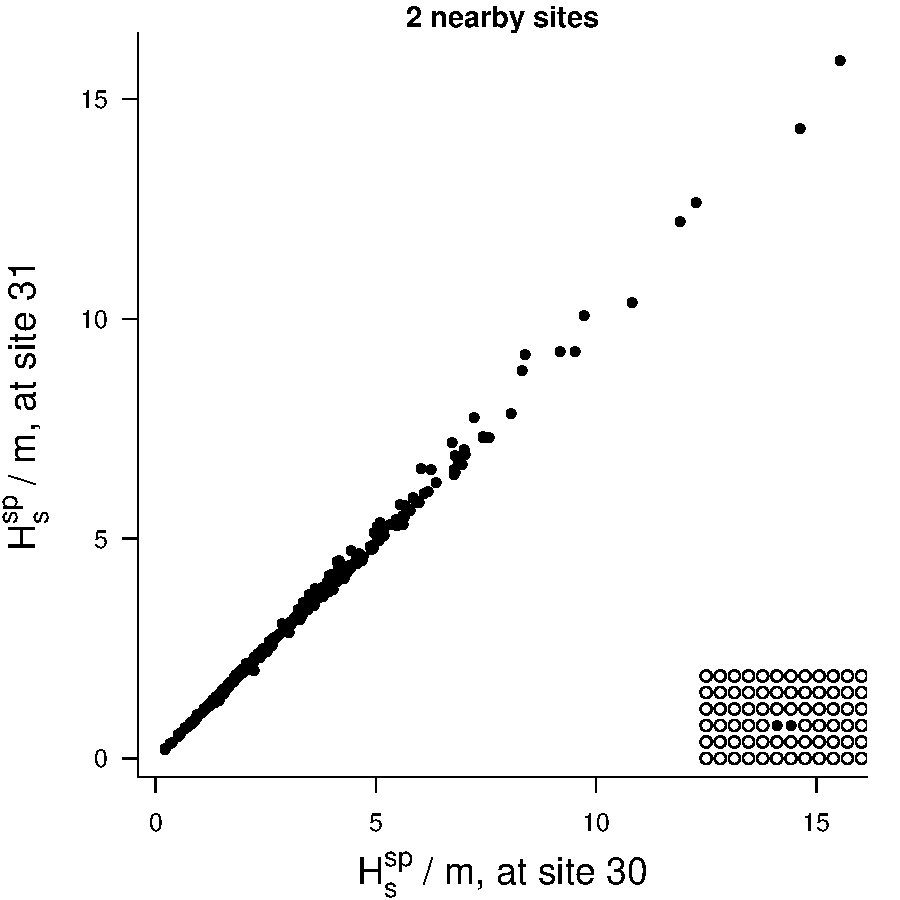
\includegraphics[width=7.5cm, angle=0]{space_dep_nearby.pdf}  % width changes size
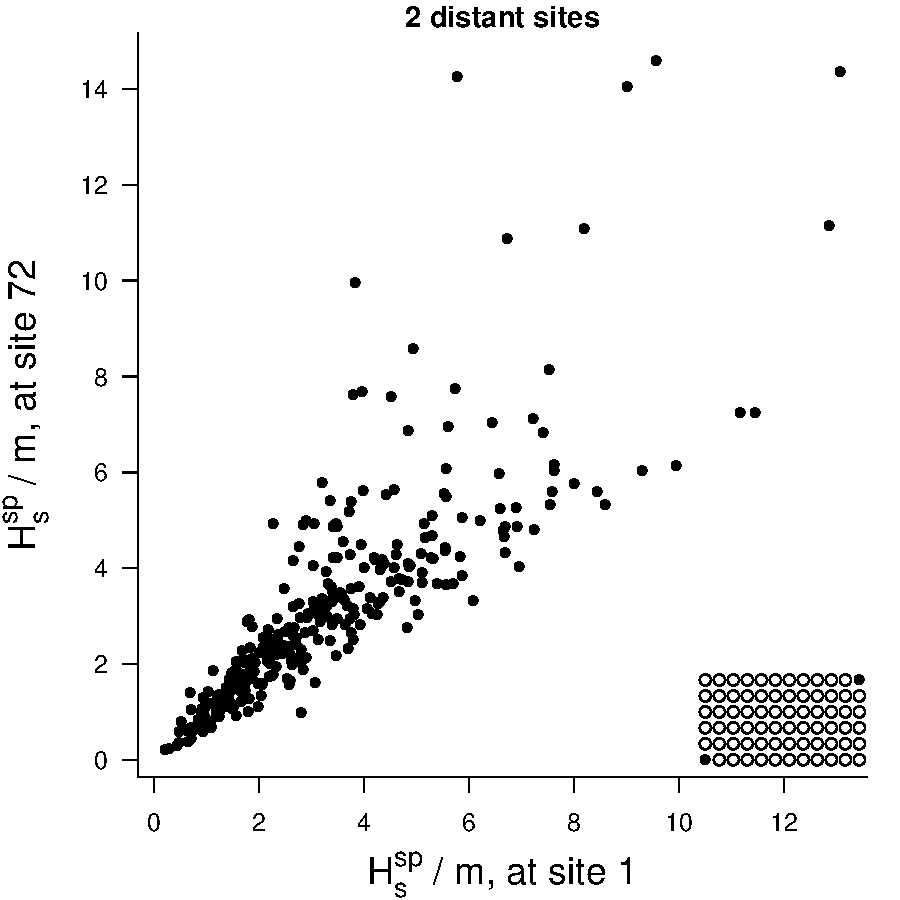
\includegraphics[width=7.5cm, angle=0]{space_dep_distant.pdf} % angle changes orientation
\vspace*{-0.25cm}    % manual adjustment of vertical spacing
\caption{Scatter plots of contemporaneous $H^{sp}_s$ values at pairs of sites.  Left: contiguous sites (site 30: latitude=3, longitude=6 and site 31: latitude=3 and longitude=7). Right: distant sites (site 1: latitude=1, longitude=1 and site 72: latitude=6, longitude=12)}          % a meaningful caption
\label{fig:space_dep}               % label for the figure
\end{figure}                        % end of figure environment

\subsection{Tables}
\label{sec:tables}
Table \ref{tab:simple} is an example of a fairly simple table.

\renewcommand{\arraystretch}{1.1} % increase the spacing factor value in {}
                                  % to increase the vertical spacing locally for the table
\begin{table}[h]                  % begin table environment (h asks LaTeX to try to put table here)
\centering
\begin{tabular}{lrcrc}            % column alignment  l (left), r (right), c (centre).
\\ \hline                         % \hline for  horizontal line
model   &  neg. log-lik & d.f. & ALRS        & $p$-value \\ \hline           % & separates columns
constant &  22763.20    &       &                &   \\                      % \\ end the current row
linear     &  22742.59    &  2   & 34.23       & $3.7 \times 10^{-8}$ \\     % $$ for maths
quadratic & 22737.09     &  3   & 20.50       & $1.3 \times 10^{-4}$ \\
cubic       & 22737.02     &  4   & 2.09         & 0.72 \\ \hline
\end{tabular}                     % end tabular environment
\caption{Summary of point process modelling in which the location parameter $\mu$ is modelled as a polynomial function of longitude and latitude and $\sigma$ and $\xi$ are constant.  The likelihood ratio tests compare the model with the model in the row above. neg. log-lik = negated maximised log-likelihood; d.f. = degrees of freedom; ALRS = adjusted likelihood ratio statistic.}
\label{tab:simple}
\end{table}
\renewcommand{\arraystretch}{1}  % set spacing factor back to 1

Table \ref{tab:more_complicated} is an example of the use of the \verb!\multicolumn! command to produce column headings that span more than one column.             %\verb!text! quotes text verbatim

\renewcommand{\arraystretch}{1.1}
\begin{table}[h]
\begin{center}
\begin{tabular}{|l|cc|cc|} \hline
                     & \multicolumn{2}{c}{wave height (m)} \vline & \multicolumn{2}{c|}{windpseed (m/s)} \\
return period  & estimate & 95\% CI & estimate & 95\% CI \\ \hline
10 years    &   \,\,\,8.7          &     (\,\,\,8.0, 10.7)  & 10.2 & (\,\,\,5.7, 14.4)  \\
100 years     &   22.1          &    (20.6, 25.6)     & 34.9 & (30.1, 42.4)  \\
1,000 years    &   35.5          &    (32.4, 42.5)    & 63.5 & (67.3, 76.9)  \\
10,000 years    &    40.3         &     (35.2, 52.8)    & 78.6 & (70.9, 98.0)  \\ \hline
\end{tabular}
\caption{Estimates and 95\% confidence intervals of return levels of $H_s$.}
\label{tab:more_complicated}
\end{center}
\end{table}
\renewcommand{\arraystretch}{1}

\subsection{Mathematics}
\label{sec:maths}
\subsubsection*{Maths in text} % subsubsection* produces no subsubsection number
Maths in text needs to be enclosed between dollar signs, e.g. \verb!$x$! gives $x$ (rather than x) and \verb!$f$! gives maths font $f$ (rather than f).

We get Greek symbols like this: $\lambda,\alpha,\beta,\gamma,\delta,\phi,\theta,\ldots$.
\ldots and mathematical operators like this: $1/x, x^{-1}, x_2,xy, \log x, 1+x, -2,x^2, \exp(x), \sin x$.

\subsubsection*{Displayed equations}

\newcommand{\e}{ {\rm e} } % a useful way to produce your own LaTeX commands

Using the \verb!equation! environment: \verb!\begin{equation}! \ldots \verb!\end{equation}!.
An exponential distribution, with mean $1/\lambda$, has probability density function (p.d.f.)
\begin{equation}
f_X(x) = \lambda \, \e^{-\lambda x}, \quad x > 0.  % \,  small space, \quad : bigger space
\label{eqn:one} % label for equation
\end{equation}
This comment refers to equation (\ref{eqn:one}).

An alternative way to produce this displayed equation is to enclose it between \verb!\[! and \verb!\]! \ldots
\[ f_X(x) = \lambda \, \e^{-\lambda x}, \quad x > 0.  \]
\ldots but no equation number is produced.

\subsubsection*{Multi-line displayed equations}
Using the \verb!align! environment (produces equation numbers) \ldots

Suppose that we have a random sample $X_1,\ldots,X_n$ from an exponential distribution with mean $1/\lambda$.
The likelihood function for $\lambda$ is given by
\begin{align}                                                                % align is part of the amsmath package
 L(\lambda) &= \prod_{i=1}^n \lambda \e^{-\lambda x_i} \notag \\             % use \notag for no equation number
 &= \lambda^n \,\e^{-\lambda \sum_{i=1}^n x_i}  \\                           % \, gives a small horizontal space
 &= \lambda^n \e^{-\lambda \displaystyle\sum_{i=1}^n x_i}  \label{eqn:two}\\ % displaystyle gives a big summation sign
 &= \lambda^n \exp \left\{-\lambda \displaystyle\sum_{i=1}^n x_i \right\}.   % \left\{ ... \right\} sizes brackets
\end{align}
Which of the above expressions do you think looks best?  Equation \eqref{eqn:two} is rather ugly...
% \eqref produces (number) (\ref would just produce number).

Using the \verb!align*! environment (produces no equation numbers) \ldots
\begin{align*}                         % align* produces no equation numbers
P(M_n \leq z)&=P(X_1 \leq z,X_2 \leq z,...,X_n \leq z)  \\
    &=P(X_1 \leq z) \times P(X_2 \leq z) \times \cdots \times P(X_n \leq z) \\
    &={F(z)}^n.
\end{align*}

Some more examples \ldots
The cumulative distribution function (c.d.f.) of a Generalized Extreme Value (GEV) distribution is given by
\[ P(X \le x) = \exp\left\{ - \left[ 1+\xi\left(\frac{x-\mu}{\sigma}\right) \right]^{-1/\xi} \right\}, \quad \mbox{for~} 1+\xi\left(\frac{x-\mu}{\sigma}\right) > 0. \]

\newcommand{\disp}{\displaystyle}   % create a shorthand for \displaystyle
\let\hat=\widehat                   % make all hats wide ones
We estimate $\theta$ using the estimator
\[ \widehat{\theta} = \disp\frac1n \frac{\disp\frac1M \disp\sum_{i=1}^M \hat{H}(Y_i)}{\disp\frac1N \disp\sum_{j=1}^N \hat{G}(Z_j)}, \]
where
\[ \hat{G}(y) = \frac1M \sum_{i=1}^M I(Y_i \leq y) \quad \mbox{and} \quad  \hat{H}(z) = \frac1N \sum_{j=1}^N I(Z_j \leq z). \]

Two examples of defining a quantity conditional on the value of another quantity. First using the cases environment \ldots
\begin{equation*}
|x|=
\begin{cases} x & \text{if $x \geq 0$,} \\      % left bracket is put in automatically
-x &\text{if $x \leq 0$.}
\end{cases}
\end{equation*}
\ldots and now using the array environment \ldots
\begin{equation*}
|x|= \left\{                                    % put in left bracket by hand
\begin{array}{rc} x & \text{if $x \geq 0$,} \\  % columns are right justified and centred respectively
-x &\text{if $x \leq 0$.}
\end{array} \right.                             % balance left bracket by a null right bracket
\end{equation*}
{\bf Note: Mathematics should read just like sentences of text, with punctuation, i.e. commas, full stops etc.}

\subsection{Lists}
\label{sec:lists}
% Some more user-defined commands ...
\newcommand{\simiid}{\,\stackrel{{\rm\tiny i.i.d.}}{\sim}\,}  % i.i.d. r.v.s
\newcommand{\simindep}{\,\stackrel{{\rm\tiny indep}}{\sim}\,} % indep r.v.s
\newcommand{\dist}{\,\stackrel{{\rm\tiny d}}{=\!=}\,}         % equality in distn

\def\approxd{\setbox0=\hbox{$\sim$}                           % approximately distributed as
\setbox1=\hbox to \wd0{\hss.\hss}%
\kern 4 pt\raise0.1ex\copy0\kern-\wd0\raise1.2ex%
\copy1\kern-\wd0\copy1\kern 4 pt}

\def\dperp{ \mathrel{\kern0pt\vbox{\hbox to 0.8em{\hss
\setbox0=\hbox{$\shortparallel$}\dp0=0pt\box0\hss}\hrule width 0.8em}}}

%\newcommand{\dist}{\,\stackrel{{\rm\tiny d}}{=}\,}
Some useful symbols presented as  bullet/numbered/lettered points using the \verb!itemize! environment \ldots
\begin{itemize}
\item $\simiid$; as in $X_1,\ldots,X_n \simiid N(\mu,\sigma^2)$.
\item [2.] $\simindep$; as in $X_i \simindep N(\mu_i,\sigma^2)$, for $i=1,\ldots,n$.
\item [(d)] $\dist$; as in $X_1 \dist X_2$, i.e. $X_1$ has the same distribution as $X_2$.
\item [(i)] $W \approxd \chi^2_p$, i.e. $W$ is approximately chi-squared with $p$ degrees of freedom.
\item $X_1 \dperp X_2$, i.e. $X_1$ is independent of $X_2$.
\end{itemize}
The \verb!enumerate! environment can be used to number items automatically using 1., 2., etc.

\subsection{Citing books, papers etc.}
\label{sec:refs}
Remember to read the guidelines on the STATG099 Moodle page.

\citet{Coles2001} is a good introduction to extreme value theory.
%citet when citation is part of a sentence

Many papers \citep{BCT2000} have also been written about exteme value theory.
% \citep when citation is in brackets.

\section{Conclusion}

\addcontentsline{toc}{section}{References} % to add references to table of contents
\bibliography{example}                     % read references from example.bib
\bibliographystyle{Chicago}                % file to determine the style of references

\end{document} 